\subsection{Spanningsreferentie}\label{sec:referenceVoltage}
De ISFET uitleesschakeling heeft een spanningsreferentie nodig om te werken. Deze spanningsreferentie is onderdeel van de uitleesschakeling van de pH sensor, en bevindt zich dus in hetzelfde blok als de uitleesschakeling zelf. Dit is te zien in \cref{fig:referenceInSchema}
\begin{figure}[!htbp]
    \centering
    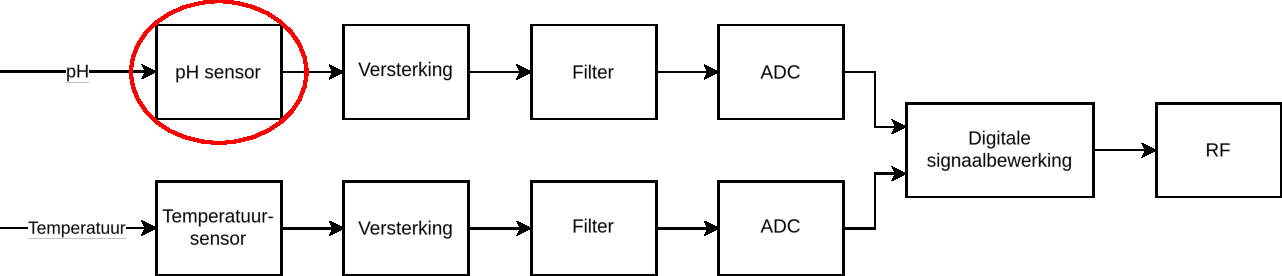
\includegraphics[width=0.95\textwidth]{signaalblokjes/pHInSchema.pdf}
    \caption{Het onderdeel van \cref{fig:analogeBewerkingsFunctie} waar de spanningsreferentie zich in bevindt.}
    \label{fig:referenceInSchema}
\end{figure}

Hiervoor is als implementatie een spanningsdeler gekozen. De schakeling van deze spanningsdeler is te zien in \cref{fig:divider}.
De condensator wordt gebruikt om ruis te verminderen op hogere frequenties, en dient ook als filter voor hoogfrequente storing in de voedingsspanning.

\begin{figure}[!htbp]
    \centering
    \def\svgwidth{0.5\textwidth}
    \subsection{Spanningsreferentie}\label{sec:referenceVoltage}

De ISFET uitleesschakeling heeft een spanningsreferentie nodig om te werken.
% TODO: Vertel misschien over andere methoden.
Hiervoor is als implementatie een spanningsdeler gekozen. De schakeling van deze spanningsdeler is te zien in \cref{fig:divider}.
De condensator wordt gebruikt om ruis te verminderen op hogere frequenties, en dient ook als filter voor hoogfrequente storing in de voedingsspanning.

\begin{figure}[!htbp]
    \centering
    \def\svgwidth{0.5\textwidth}
    \subsection{Spanningsreferentie}\label{sec:referenceVoltage}

De ISFET uitleesschakeling heeft een spanningsreferentie nodig om te werken.
% TODO: Vertel misschien over andere methoden.
Hiervoor is als implementatie een spanningsdeler gekozen. De schakeling van deze spanningsdeler is te zien in \cref{fig:divider}.
De condensator wordt gebruikt om ruis te verminderen op hogere frequenties, en dient ook als filter voor hoogfrequente storing in de voedingsspanning.

\begin{figure}[!htbp]
    \centering
    \def\svgwidth{0.5\textwidth}
    \subsection{Spanningsreferentie}\label{sec:referenceVoltage}

De ISFET uitleesschakeling heeft een spanningsreferentie nodig om te werken.
% TODO: Vertel misschien over andere methoden.
Hiervoor is als implementatie een spanningsdeler gekozen. De schakeling van deze spanningsdeler is te zien in \cref{fig:divider}.
De condensator wordt gebruikt om ruis te verminderen op hogere frequenties, en dient ook als filter voor hoogfrequente storing in de voedingsspanning.

\begin{figure}[!htbp]
    \centering
    \def\svgwidth{0.5\textwidth}
    \input{img/divider.pdf_tex}
    \caption{De schakeling van de spanningsdeler die dient als spanningsreferentie.}
    \label{fig:divider}
\end{figure}

De overdracht van deze spanningsdeler is te vinden in \cref{eq:dividerTransfer}.
\begin{equation}\label{eq:dividerTransfer}
    H(s) = \frac{U_{ref}(s)}{U_{dd}(s)} = \frac{R_2}{R_1 + R_2 + R_2Cs}
\end{equation}

\subsubsection{Vermogen}
Het vermogen dat de spanningsdeler dissipeert, kan met \cref{eq:dividerPower} berekend worden.
\begin{equation}\label{eq:dividerPower}
    P(s) = U_{dd}^2(s)\frac{1+R_2Cs}{R_1 + R_2 + R_1R_2Cs}
    \tagaddtext{[\si{\watt}]}
\end{equation}
Met een constante DC ingangsspanning kan dit vereenvoudigd worden naar \cref{eq:dividerPowerSimple}.
\begin{equation}\label{eq:dividerPowerSimple}
    P = \frac{U_{dd}^2}{R_1 + R_2}
    \tagaddtext{[\si{\watt}]}
\end{equation}

\subsubsection{Ruis}
Om de ruis van deze schakeling te berekenen moet een aantal stappen genomen worden. Aangezien de ingangsbron $U_{dd}$ een spanningsbron is, kan deze als kortsluiting genomen worden. Op deze manier kunnen de twee weerstanden parallel genomen worden, en verandert de schakeling in een simpel RC filter. In \cref{fig:dividerNoise} is deze omgebouwde schakeling te zien.

\begin{figure}[!htbp]
    \centering
    \def\svgwidth{0.35\textwidth}
    \input{img/dividerNoise.pdf_tex}
    \caption{De omgebouwde schakeling om ruis mee te berekenen.}
    \label{fig:dividerNoise}
\end{figure}

\noindent
Voor de spectrale spanningsruisdichtheid aan de uitgang $U_{ref}$ kan \cref{eq:dividerNoiseLaplace} worden opgesteld.
\begin{equation}\label{eq:dividerNoiseLaplace}
    S_{n,u_{ref}} = 4kTR_e\left(\frac{1}{1 + R_eCs}\right)^2
    \tagaddtext{[\si{\volt\squared\per\hertz}]}
\end{equation}
Wanneer de absolute waarde van de ruis wordt genomen, kan deze over de bandbreedte geïntegreerd worden. Dit resulteert in \cref{eq:dividerNoiseInt}, waar B de bandbreedte is.
\begin{equation}\label{eq:dividerNoiseInt}
    u_{n,ref}^2 = 4kTR_e\int_{B} \frac{1}{1 + (2\pi f R_e C)^2} df
    \tagaddtext{[\si{\volt\squared}]}
\end{equation}
Met een oneindige bandbreedte komt deze integraal uit op \cref{eq:dividerNoiseIntegratedInf}.
\begin{equation}\label{eq:dividerNoiseIntegratedInf}
    u_{n,ref}^2 = \lim_{f\rightarrow\infty}\frac{2kT}{\pi C} \arctan(2\pi f R_eC)
    \tagaddtext{[\si{\volt\squared}]}
\end{equation}
Aangezien de inverse tangens $\frac{\pi}{2}$ nadert, komt dit limiet uit op \cref{eq:dividerNoise}.
\begin{equation}\label{eq:dividerNoise}
    u_{n,ref}^2 = \frac{kT}{C}
    \tagaddtext{[\si{\volt\squared}]}
\end{equation}
Omdat een oneindige bandbreedte gebruikt is om op \cref{eq:dividerNoise} te komen, berekend deze de ruis in het ergste geval. De weerstandswaardes van $R_1$ en $R_2$ zijn hierbij irrelevant. Hierdoor is ruis geen bepalende factor meer tijdens het kiezen van de weerstandswaardes van de spanningsdeler, en kunnen deze volledig gebaseerd worden op vermogensverbruik. Volgens \cref{eq:dividerPowerSimple} is het vermogen omgekeerd evenredig met de som van de weerstandswaardes. Daarbij zit de uitgang van de spanningsdeler direct verbonden met de ingang van een nullor. Er hoeft dus geen rekening gehouden te worden met de uitgangsimpedantie van de spanningsbron. Hierdoor is het voor het vermogensverbruik voordelig om de weerstandswaardes zo hoog mogelijk te kiezen.

\subsubsection{Simulatie}

Om te verifiëren dat de spanningsreferentie goed werkt, is er een aantal simulaties uitgevoerd.

In \cref{fig:referenceSimFreq} is het resultaat van een AC simulatie te zien. Hier is $H(f)$ de overdracht van $U_{dd}$ naar

\begin{figure}[!htbp]
    \centering
    \pgfplotsset{width=0.7\textwidth}
    \input{plots/referenceSimFreq.tex}
    \caption{Het resultaat van een AC simulatie van de spanningsreferentie.}
    \label{fig:referenceSimFreq}
\end{figure}


\begin{figure}[!htbp]
    \centering
    \pgfplotsset{width=0.7\textwidth}
    \input{plots/referenceSimTrans.tex}
    \caption{Het resultaat van een transient simulatie van de spanningsreferentie.}
    \label{fig:referenceSimTrans}
\end{figure}


\begin{figure}[!htbp]
    \centering
    \pgfplotsset{width=0.7\textwidth}
    \input{plots/referenceSimNoise.tex}
    \caption{Het resultaat van een ruissimulatie van de spanningsreferentie.}
    \label{fig:referenceSimNoise}
\end{figure}

% 64nV aan ruis
    \caption{De schakeling van de spanningsdeler die dient als spanningsreferentie.}
    \label{fig:divider}
\end{figure}

De overdracht van deze spanningsdeler is te vinden in \cref{eq:dividerTransfer}.
\begin{equation}\label{eq:dividerTransfer}
    H(s) = \frac{U_{ref}(s)}{U_{dd}(s)} = \frac{R_2}{R_1 + R_2 + R_2Cs}
\end{equation}

\subsubsection{Vermogen}
Het vermogen dat de spanningsdeler dissipeert, kan met \cref{eq:dividerPower} berekend worden.
\begin{equation}\label{eq:dividerPower}
    P(s) = U_{dd}^2(s)\frac{1+R_2Cs}{R_1 + R_2 + R_1R_2Cs}
    \tagaddtext{[\si{\watt}]}
\end{equation}
Met een constante DC ingangsspanning kan dit vereenvoudigd worden naar \cref{eq:dividerPowerSimple}.
\begin{equation}\label{eq:dividerPowerSimple}
    P = \frac{U_{dd}^2}{R_1 + R_2}
    \tagaddtext{[\si{\watt}]}
\end{equation}

\subsubsection{Ruis}
Om de ruis van deze schakeling te berekenen moet een aantal stappen genomen worden. Aangezien de ingangsbron $U_{dd}$ een spanningsbron is, kan deze als kortsluiting genomen worden. Op deze manier kunnen de twee weerstanden parallel genomen worden, en verandert de schakeling in een simpel RC filter. In \cref{fig:dividerNoise} is deze omgebouwde schakeling te zien.

\begin{figure}[!htbp]
    \centering
    \def\svgwidth{0.35\textwidth}
    \begin{tikzpicture}
    \pgfplotsset{width=\textwidth}
    \newcommand\BOLZ{1.380649e-23}
    \newcommand\TEMP{300}
    \newcommand\OMEGAC{15*2*pi}
    \newcommand\RESRAT{(7/11)}
    \newcommand\REQU{(1/(1/x + \RESRAT/x))}
    \newcommand\CAP{0.000001}

    \pgfplotsset{set layers}
    \begin{axis}[
        xmode=log,
        ymode=log,
        xlabel={$R_1 [\si{\ohm}]$},
        ylabel={$u_{n,out} [\si{\volt}]$},
        xmin=1e3, xmax=2e6,
        grid=major
    ]

    \addplot [
        red,
        domain=1e3:2e6,
        samples=201
    ]
    {sqrt((4 * \BOLZ * \TEMP / \CAP) * rad(atan(\REQU * \CAP * \OMEGAC)))};
    \end{axis}
\end{tikzpicture}
    \caption{De omgebouwde schakeling om ruis mee te berekenen.}
    \label{fig:dividerNoise}
\end{figure}

\noindent
Voor de spectrale spanningsruisdichtheid aan de uitgang $U_{ref}$ kan \cref{eq:dividerNoiseLaplace} worden opgesteld.
\begin{equation}\label{eq:dividerNoiseLaplace}
    S_{n,u_{ref}} = 4kTR_e\left(\frac{1}{1 + R_eCs}\right)^2
    \tagaddtext{[\si{\volt\squared\per\hertz}]}
\end{equation}
Wanneer de absolute waarde van de ruis wordt genomen, kan deze over de bandbreedte geïntegreerd worden. Dit resulteert in \cref{eq:dividerNoiseInt}, waar B de bandbreedte is.
\begin{equation}\label{eq:dividerNoiseInt}
    u_{n,ref}^2 = 4kTR_e\int_{B} \frac{1}{1 + (2\pi f R_e C)^2} df
    \tagaddtext{[\si{\volt\squared}]}
\end{equation}
Met een oneindige bandbreedte komt deze integraal uit op \cref{eq:dividerNoiseIntegratedInf}.
\begin{equation}\label{eq:dividerNoiseIntegratedInf}
    u_{n,ref}^2 = \lim_{f\rightarrow\infty}\frac{2kT}{\pi C} \arctan(2\pi f R_eC)
    \tagaddtext{[\si{\volt\squared}]}
\end{equation}
Aangezien de inverse tangens $\frac{\pi}{2}$ nadert, komt dit limiet uit op \cref{eq:dividerNoise}.
\begin{equation}\label{eq:dividerNoise}
    u_{n,ref}^2 = \frac{kT}{C}
    \tagaddtext{[\si{\volt\squared}]}
\end{equation}
Omdat een oneindige bandbreedte gebruikt is om op \cref{eq:dividerNoise} te komen, berekend deze de ruis in het ergste geval. De weerstandswaardes van $R_1$ en $R_2$ zijn hierbij irrelevant. Hierdoor is ruis geen bepalende factor meer tijdens het kiezen van de weerstandswaardes van de spanningsdeler, en kunnen deze volledig gebaseerd worden op vermogensverbruik. Volgens \cref{eq:dividerPowerSimple} is het vermogen omgekeerd evenredig met de som van de weerstandswaardes. Daarbij zit de uitgang van de spanningsdeler direct verbonden met de ingang van een nullor. Er hoeft dus geen rekening gehouden te worden met de uitgangsimpedantie van de spanningsbron. Hierdoor is het voor het vermogensverbruik voordelig om de weerstandswaardes zo hoog mogelijk te kiezen.

\subsubsection{Simulatie}

Om te verifiëren dat de spanningsreferentie goed werkt, is er een aantal simulaties uitgevoerd.

In \cref{fig:referenceSimFreq} is het resultaat van een AC simulatie te zien. Hier is $H(f)$ de overdracht van $U_{dd}$ naar

\begin{figure}[!htbp]
    \centering
    \pgfplotsset{width=0.7\textwidth}
    \begin{tikzpicture}
    \tikzset{
        small dot/.style={fill=black,circle,scale=0.4,thick},
    }

    \begin{axis}[
        xmode=log,
        xlabel={$f$ [\unit{\hertz}]},
        ylabel={$H(f)$ [\unit{\decibel}]},
        grid=major,
        height=6cm
    ]
        \addplot [
            mark=none,
            line width=0.5mm
        ] table[x=freq,y=out] {sim/referenceSimFreq.dat};
        % \addplot [
        %     red,
        %     mark=*
        % ] coordinates {(0.18714337, -19.391)};
        \node [small dot,pin={[pin edge={line width=0.3mm,black}]0:kantelpunt}] at (0.18714337, -19.391) {};
    \end{axis}
\end{tikzpicture}


    \caption{Het resultaat van een AC simulatie van de spanningsreferentie.}
    \label{fig:referenceSimFreq}
\end{figure}


\begin{figure}[!htbp]
    \centering
    \pgfplotsset{width=0.7\textwidth}
    \begin{tikzpicture}
    \tikzset{
        small dot/.style={fill=black,circle,scale=0.4},
    }

    \begin{axis}[
        xlabel={$t$ [\unit{\second}]},
        ylabel={$U_{ref}$ [\unit{\volt}]},
        ytick       ={0,0.05,0.1,0.15},
        yticklabels ={0,0.05,0.1,0.15},
        grid=major,
        height=6cm,
    ]
        \addplot [
            mark=none,
            line width=0.5mm
        ] table[x=time,y=out] {sim/referenceSimTrans.dat};
        \node [small dot,pin={[pin edge={line width=0.3mm,black}]0:Voeding wordt geactiveerd}] at (1,0) {};
    \end{axis}


\end{tikzpicture}


    \caption{Het resultaat van een transient simulatie van de spanningsreferentie.}
    \label{fig:referenceSimTrans}
\end{figure}


\begin{figure}[!htbp]
    \centering
    \pgfplotsset{width=0.7\textwidth}
    \begin{tikzpicture}

    \begin{axis}[
        xmode=log,
        xlabel={$f$ [\unit{\hertz}]},
        ylabel={$\sqrt{S_{u,n}} \,\,\,\, \left[\unit{\nano\volt}/\sqrt{\unit{\hertz}}\right]$},
        grid=major,
        height=6cm
    ]
    \addplot [
        mark=none,
        line width=0.5mm,
        y filter/.code={\pgfmathparse{#1*1e9}\pgfmathresult}
    ] table[x=freq,y=noise] {sim/referenceSimNoise.dat};
    \end{axis}
\end{tikzpicture}


    \caption{Het resultaat van een ruissimulatie van de spanningsreferentie.}
    \label{fig:referenceSimNoise}
\end{figure}

% 64nV aan ruis
    \caption{De schakeling van de spanningsdeler die dient als spanningsreferentie.}
    \label{fig:divider}
\end{figure}

De overdracht van deze spanningsdeler is te vinden in \cref{eq:dividerTransfer}.
\begin{equation}\label{eq:dividerTransfer}
    H(s) = \frac{U_{ref}(s)}{U_{dd}(s)} = \frac{R_2}{R_1 + R_2 + R_2Cs}
\end{equation}

\subsubsection{Vermogen}
Het vermogen dat de spanningsdeler dissipeert, kan met \cref{eq:dividerPower} berekend worden.
\begin{equation}\label{eq:dividerPower}
    P(s) = U_{dd}^2(s)\frac{1+R_2Cs}{R_1 + R_2 + R_1R_2Cs}
    \tagaddtext{[\si{\watt}]}
\end{equation}
Met een constante DC ingangsspanning kan dit vereenvoudigd worden naar \cref{eq:dividerPowerSimple}.
\begin{equation}\label{eq:dividerPowerSimple}
    P = \frac{U_{dd}^2}{R_1 + R_2}
    \tagaddtext{[\si{\watt}]}
\end{equation}

\subsubsection{Ruis}
Om de ruis van deze schakeling te berekenen moet een aantal stappen genomen worden. Aangezien de ingangsbron $U_{dd}$ een spanningsbron is, kan deze als kortsluiting genomen worden. Op deze manier kunnen de twee weerstanden parallel genomen worden, en verandert de schakeling in een simpel RC filter. In \cref{fig:dividerNoise} is deze omgebouwde schakeling te zien.

\begin{figure}[!htbp]
    \centering
    \def\svgwidth{0.35\textwidth}
    \begin{tikzpicture}
    \pgfplotsset{width=\textwidth}
    \newcommand\BOLZ{1.380649e-23}
    \newcommand\TEMP{300}
    \newcommand\OMEGAC{15*2*pi}
    \newcommand\RESRAT{(7/11)}
    \newcommand\REQU{(1/(1/x + \RESRAT/x))}
    \newcommand\CAP{0.000001}

    \pgfplotsset{set layers}
    \begin{axis}[
        xmode=log,
        ymode=log,
        xlabel={$R_1 [\si{\ohm}]$},
        ylabel={$u_{n,out} [\si{\volt}]$},
        xmin=1e3, xmax=2e6,
        grid=major
    ]

    \addplot [
        red,
        domain=1e3:2e6,
        samples=201
    ]
    {sqrt((4 * \BOLZ * \TEMP / \CAP) * rad(atan(\REQU * \CAP * \OMEGAC)))};
    \end{axis}
\end{tikzpicture}
    \caption{De omgebouwde schakeling om ruis mee te berekenen.}
    \label{fig:dividerNoise}
\end{figure}

\noindent
Voor de spectrale spanningsruisdichtheid aan de uitgang $U_{ref}$ kan \cref{eq:dividerNoiseLaplace} worden opgesteld.
\begin{equation}\label{eq:dividerNoiseLaplace}
    S_{n,u_{ref}} = 4kTR_e\left(\frac{1}{1 + R_eCs}\right)^2
    \tagaddtext{[\si{\volt\squared\per\hertz}]}
\end{equation}
Wanneer de absolute waarde van de ruis wordt genomen, kan deze over de bandbreedte geïntegreerd worden. Dit resulteert in \cref{eq:dividerNoiseInt}, waar B de bandbreedte is.
\begin{equation}\label{eq:dividerNoiseInt}
    u_{n,ref}^2 = 4kTR_e\int_{B} \frac{1}{1 + (2\pi f R_e C)^2} df
    \tagaddtext{[\si{\volt\squared}]}
\end{equation}
Met een oneindige bandbreedte komt deze integraal uit op \cref{eq:dividerNoiseIntegratedInf}.
\begin{equation}\label{eq:dividerNoiseIntegratedInf}
    u_{n,ref}^2 = \lim_{f\rightarrow\infty}\frac{2kT}{\pi C} \arctan(2\pi f R_eC)
    \tagaddtext{[\si{\volt\squared}]}
\end{equation}
Aangezien de inverse tangens $\frac{\pi}{2}$ nadert, komt dit limiet uit op \cref{eq:dividerNoise}.
\begin{equation}\label{eq:dividerNoise}
    u_{n,ref}^2 = \frac{kT}{C}
    \tagaddtext{[\si{\volt\squared}]}
\end{equation}
Omdat een oneindige bandbreedte gebruikt is om op \cref{eq:dividerNoise} te komen, berekend deze de ruis in het ergste geval. De weerstandswaardes van $R_1$ en $R_2$ zijn hierbij irrelevant. Hierdoor is ruis geen bepalende factor meer tijdens het kiezen van de weerstandswaardes van de spanningsdeler, en kunnen deze volledig gebaseerd worden op vermogensverbruik. Volgens \cref{eq:dividerPowerSimple} is het vermogen omgekeerd evenredig met de som van de weerstandswaardes. Daarbij zit de uitgang van de spanningsdeler direct verbonden met de ingang van een nullor. Er hoeft dus geen rekening gehouden te worden met de uitgangsimpedantie van de spanningsbron. Hierdoor is het voor het vermogensverbruik voordelig om de weerstandswaardes zo hoog mogelijk te kiezen.

\subsubsection{Simulatie}

Om te verifiëren dat de spanningsreferentie goed werkt, is er een aantal simulaties uitgevoerd.

In \cref{fig:referenceSimFreq} is het resultaat van een AC simulatie te zien. Hier is $H(f)$ de overdracht van $U_{dd}$ naar

\begin{figure}[!htbp]
    \centering
    \pgfplotsset{width=0.7\textwidth}
    \begin{tikzpicture}
    \tikzset{
        small dot/.style={fill=black,circle,scale=0.4,thick},
    }

    \begin{axis}[
        xmode=log,
        xlabel={$f$ [\unit{\hertz}]},
        ylabel={$H(f)$ [\unit{\decibel}]},
        grid=major,
        height=6cm
    ]
        \addplot [
            mark=none,
            line width=0.5mm
        ] table[x=freq,y=out] {sim/referenceSimFreq.dat};
        % \addplot [
        %     red,
        %     mark=*
        % ] coordinates {(0.18714337, -19.391)};
        \node [small dot,pin={[pin edge={line width=0.3mm,black}]0:kantelpunt}] at (0.18714337, -19.391) {};
    \end{axis}
\end{tikzpicture}


    \caption{Het resultaat van een AC simulatie van de spanningsreferentie.}
    \label{fig:referenceSimFreq}
\end{figure}


\begin{figure}[!htbp]
    \centering
    \pgfplotsset{width=0.7\textwidth}
    \begin{tikzpicture}
    \tikzset{
        small dot/.style={fill=black,circle,scale=0.4},
    }

    \begin{axis}[
        xlabel={$t$ [\unit{\second}]},
        ylabel={$U_{ref}$ [\unit{\volt}]},
        ytick       ={0,0.05,0.1,0.15},
        yticklabels ={0,0.05,0.1,0.15},
        grid=major,
        height=6cm,
    ]
        \addplot [
            mark=none,
            line width=0.5mm
        ] table[x=time,y=out] {sim/referenceSimTrans.dat};
        \node [small dot,pin={[pin edge={line width=0.3mm,black}]0:Voeding wordt geactiveerd}] at (1,0) {};
    \end{axis}


\end{tikzpicture}


    \caption{Het resultaat van een transient simulatie van de spanningsreferentie.}
    \label{fig:referenceSimTrans}
\end{figure}


\begin{figure}[!htbp]
    \centering
    \pgfplotsset{width=0.7\textwidth}
    \begin{tikzpicture}

    \begin{axis}[
        xmode=log,
        xlabel={$f$ [\unit{\hertz}]},
        ylabel={$\sqrt{S_{u,n}} \,\,\,\, \left[\unit{\nano\volt}/\sqrt{\unit{\hertz}}\right]$},
        grid=major,
        height=6cm
    ]
    \addplot [
        mark=none,
        line width=0.5mm,
        y filter/.code={\pgfmathparse{#1*1e9}\pgfmathresult}
    ] table[x=freq,y=noise] {sim/referenceSimNoise.dat};
    \end{axis}
\end{tikzpicture}


    \caption{Het resultaat van een ruissimulatie van de spanningsreferentie.}
    \label{fig:referenceSimNoise}
\end{figure}

% 64nV aan ruis
    \caption{De schakeling van de spanningsdeler die dient als spanningsreferentie.}
    \label{fig:divider}
\end{figure}

De overdracht van deze spanningsdeler is te vinden in \cref{eq:dividerTransfer}.
\begin{equation}\label{eq:dividerTransfer}
    H(s) = \frac{U_{ref}(s)}{U_{dd}(s)} = \frac{R_2}{R_1 + R_2 + R_2Cs}
\end{equation}

\subsubsection{Vermogen}
Het vermogen dat de spanningsdeler dissipeert, kan met \cref{eq:dividerPower} berekend worden.
\begin{equation}\label{eq:dividerPower}
    P(s) = U_{dd}^2(s)\frac{1+R_2Cs}{R_1 + R_2 + R_1R_2Cs}
    \tagaddtext{[\si{\watt}]}
\end{equation}
Met een constante DC ingangsspanning kan dit vereenvoudigd worden naar \cref{eq:dividerPowerSimple}.
\begin{equation}\label{eq:dividerPowerSimple}
    P = \frac{U_{dd}^2}{R_1 + R_2}
    \tagaddtext{[\si{\watt}]}
\end{equation}

\subsubsection{Ruis}
Om de ruis van deze schakeling te berekenen moet een aantal stappen genomen worden. Aangezien de ingangsbron $U_{dd}$ een spanningsbron is, kan deze als kortsluiting genomen worden. Op deze manier kunnen de twee weerstanden parallel genomen worden, en verandert de schakeling in een simpel RC filter. In \cref{fig:dividerNoise} is deze omgebouwde schakeling te zien.

\begin{figure}[!htbp]
    \centering
    \def\svgwidth{0.35\textwidth}
    \begin{tikzpicture}
    \pgfplotsset{width=\textwidth}
    \newcommand\BOLZ{1.380649e-23}
    \newcommand\TEMP{300}
    \newcommand\OMEGAC{15*2*pi}
    \newcommand\RESRAT{(7/11)}
    \newcommand\REQU{(1/(1/x + \RESRAT/x))}
    \newcommand\CAP{0.000001}

    \pgfplotsset{set layers}
    \begin{axis}[
        xmode=log,
        ymode=log,
        xlabel={$R_1 [\si{\ohm}]$},
        ylabel={$u_{n,out} [\si{\volt}]$},
        xmin=1e3, xmax=2e6,
        grid=major
    ]

    \addplot [
        red,
        domain=1e3:2e6,
        samples=201
    ]
    {sqrt((4 * \BOLZ * \TEMP / \CAP) * rad(atan(\REQU * \CAP * \OMEGAC)))};
    \end{axis}
\end{tikzpicture}
    \caption{De omgebouwde schakeling om ruis mee te berekenen.}
    \label{fig:dividerNoise}
\end{figure}

\noindent
Voor de spectrale spanningsruisdichtheid aan de uitgang $U_{ref}$ kan \cref{eq:dividerNoiseLaplace} worden opgesteld.
\begin{equation}\label{eq:dividerNoiseLaplace}
    S_{n,u_{ref}} = 4kTR_e\left(\frac{1}{1 + R_eCs}\right)^2
    \tagaddtext{[\si{\volt\squared\per\hertz}]}
\end{equation}
Wanneer de absolute waarde van de ruis wordt genomen, kan deze over de bandbreedte geïntegreerd worden. Dit resulteert in \cref{eq:dividerNoiseInt}, waar B de bandbreedte is.
\begin{equation}\label{eq:dividerNoiseInt}
    u_{n,ref}^2 = 4kTR_e\int_{B} \frac{1}{1 + (2\pi f R_e C)^2} df
    \tagaddtext{[\si{\volt\squared}]}
\end{equation}
Met een oneindige bandbreedte komt deze integraal uit op \cref{eq:dividerNoiseIntegratedInf}.
\begin{equation}\label{eq:dividerNoiseIntegratedInf}
    u_{n,ref}^2 = \lim_{f\rightarrow\infty}\frac{2kT}{\pi C} \arctan(2\pi f R_eC)
    \tagaddtext{[\si{\volt\squared}]}
\end{equation}
Aangezien de inverse tangens $\frac{\pi}{2}$ nadert, komt dit limiet uit op \cref{eq:dividerNoise}.
\begin{equation}\label{eq:dividerNoise}
    u_{n,ref}^2 = \frac{kT}{C}
    \tagaddtext{[\si{\volt\squared}]}
\end{equation}
Omdat een oneindige bandbreedte gebruikt is om op \cref{eq:dividerNoise} te komen, berekend deze de ruis in het ergste geval. De weerstandswaardes van $R_1$ en $R_2$ zijn hierbij irrelevant. Hierdoor is ruis geen bepalende factor meer tijdens het kiezen van de weerstandswaardes van de spanningsdeler, en kunnen deze volledig gebaseerd worden op vermogensverbruik. Volgens \cref{eq:dividerPowerSimple} is het vermogen omgekeerd evenredig met de som van de weerstandswaardes. Daarbij zit de uitgang van de spanningsdeler direct verbonden met de ingang van een nullor. Er hoeft dus geen rekening gehouden te worden met de uitgangsimpedantie van de spanningsbron. Hierdoor is het voor het vermogensverbruik voordelig om de weerstandswaardes zo hoog mogelijk te kiezen.
